\documentclass{beamer}
\mode<presentation>
\usepackage{amsmath}
\usepackage{amssymb}
%\usepackage{advdate}
\usepackage{adjustbox}
\usepackage{subcaption}
\usepackage{enumitem}
\usepackage{multicol}
\usepackage{gensymb}
\usepackage{mathtools}
\usepackage{listings}
\usepackage{url}
\def\UrlBreaks{\do\/\do-}
\usetheme{Boadilla}
\usecolortheme{lily}
\setbeamertemplate{footline}
{
  \leavevmode%
  \hbox{%
  \begin{beamercolorbox}[wd=\paperwidth,ht=2ex,dp=1ex,right]{author in head/foot}%
    \insertframenumber{} / \inserttotalframenumber\hspace*{2ex} 
  \end{beamercolorbox}}%
  \vskip0pt%
}
\setbeamertemplate{navigation symbols}{}

\providecommand{\nCr}[2]{\,^{#1}C_{#2}} % nCr
\providecommand{\nPr}[2]{\,^{#1}P_{#2}} % nPr
\providecommand{\mbf}{\mathbf}
\providecommand{\pr}[1]{\ensuremath{\Pr\left(#1\right)}}
\providecommand{\qfunc}[1]{\ensuremath{Q\left(#1\right)}}
\providecommand{\sbrak}[1]{\ensuremath{{}\left[#1\right]}}
\providecommand{\lsbrak}[1]{\ensuremath{{}\left[#1\right.}}
\providecommand{\rsbrak}[1]{\ensuremath{{}\left.#1\right]}}
\providecommand{\brak}[1]{\ensuremath{\left(#1\right)}}
\providecommand{\lbrak}[1]{\ensuremath{\left(#1\right.}}
\providecommand{\rbrak}[1]{\ensuremath{\left.#1\right)}}
\providecommand{\cbrak}[1]{\ensuremath{\left\{#1\right\}}}
\providecommand{\lcbrak}[1]{\ensuremath{\left\{#1\right.}}
\providecommand{\rcbrak}[1]{\ensuremath{\left.#1\right\}}}
\theoremstyle{remark}
\newtheorem{rem}{Remark}
\newcommand{\sgn}{\mathop{\mathrm{sgn}}}
\providecommand{\abs}[1]{\left\vert#1\right\vert}
\providecommand{\res}[1]{\Res\displaylimits_{#1}} 
\providecommand{\norm}[1]{\lVert#1\rVert}
\providecommand{\mtx}[1]{\mathbf{#1}}
\providecommand{\mean}[1]{E\left[ #1 \right]}
\providecommand{\fourier}{\overset{\mathcal{F}}{ \rightleftharpoons}}
%\providecommand{\hilbert}{\overset{\mathcal{H}}{ \rightleftharpoons}}
\providecommand{\system}{\overset{\mathcal{H}}{ \longleftrightarrow}}
	%\newcommand{\solution}[2]{\textbf{Solution:}{#1}}
%\newcommand{\solution}{\noindent \textbf{Solution: }}
\providecommand{\dec}[2]{\ensuremath{\overset{#1}{\underset{#2}{\gtrless}}}}
\newcommand{\myvec}[1]{\ensuremath{\begin{pmatrix}#1\end{pmatrix}}}
\let\vec\mathbf

\lstset{
%language=C,
frame=single, 
breaklines=true,
columns=fullflexible
}

\numberwithin{equation}{section}

\title{10.4.1.1.8 Presentation}
\author{G. Abhimanyu Koushik \\ EE24BTECH11024}

\date{\today} 
\begin{document}

\begin{frame}
\titlepage
\end{frame}

\section*{Outline}
\begin{frame}
\tableofcontents
\end{frame}
\section{Problem}
\begin{frame}
\frametitle{Problem Statement}
%
Find the roots of the equation $x^3 - 4x^2 - x + 1 = \brak{x - 2}^3$
%
\end{frame}

%\subsection{Literature}
\section{Solution}
\subsection{Theoritical Solution}
\begin{frame}
\frametitle{Theoritical Solution}
%\framesubtitle{Literature}
The given equation can be simplified to
\begin{align}
	x^3 - 4x^2 - x + 1 &= \brak{x - 2}^3\\
	x^3 - 4x^2 - x + 1 &= x^3-6x^2+12x-8\\
	2x^2 - 13x + 9 &= 0
\end{align}
Applying quadratic formula gives solution as
\begin{align}
	x_1 = \frac{13-\sqrt{97}}{4}\\
	x_2 = \frac{13+\sqrt{97}}{4}
\end{align}
\end{frame}
\subsection{Computational Solution}
\begin{frame}
\frametitle{Computational Solution}
Two methods to find solution of a quadratic equation are:\\
Matrix-Based Method:\\
For a polynomial equation of form $x_n+b_{n-1}x^{n-1}+\dots+b_2x^2+b_1x+b_0 = 0$ we construct a matrix called companion matrix of form
\begin{align}
	\Lambda = \myvec{0&1&0&\dots&0\\ 0&0&1&\dots&0\\ \vdots &\vdots &\vdots &\ddots&\vdots\\0&0&0&\vdots&1\\-b_0&-b_1&-b_2&\dots&-b_{n-1}}
\end{align}
The eigenvalues of this matrix are the roots of the given polynomial equation.\\
The solution given by the code is
\begin{align}
	x_1 = 0.7878\\
	x_2 = 5.7122
\end{align}
\end{frame}
\begin{frame}
Newton-Raphson Method:\\
Start with an initial guess $x_0$, and then run the following logical loop,
\begin{align}
    x_{n+1} = x_n - \frac{f\brak{x_n}}{f^{\prime}\brak{x_n}} 
\end{align}
where,
\begin{align}
    f\brak{x} = 2x^2 - 13x + 9\\
    f^{\prime}\brak{x} = 4x-13
\end{align}
The update equation will be
\begin{align}
	x_{n+1} = x_n - \frac{2{x_n}^2 - 13x_n + 9}{4x_n-13}\\
\end{align}
\end{frame}
\begin{frame}
The problem with this method is if the roots are complex but the coeffcients are real, $x_n$ either converges to an extrema or grows continuously without any bound.
To get the complex solutions, however , we can just take the initial guess point to be a 
random complex number.\\
The output of a program written to find roots is shown below:
\begin{align}
	r_1 = 0.7878\\
	r_2 = 5.7122
\end{align}
\end{frame}
\begin{frame}
Companion matrix
\begin{align}
\Lambda_{0} &= \myvec{0 & 1\\-\frac{9}{2} & \frac{13}{2}}
\end{align}
The update equation will be
\begin{align}
\Lambda_{n+1} &= Q\brak{\Lambda_{n}-\sigma I}Q^\top + \sigma I\\
\end{align}
As $n$ tends to infinite, $\Lambda$ converges to Upper triangular matrix
\begin{align}
\sigma &= \frac{13}{2}\\
\Lambda_{\text{shifted}} &= \myvec{0 & 1\\-\frac{9}{2} & \frac{13}{2}} - \sigma I\\
\Lambda_{\text{shifted}} &= \myvec{\frac{-13}{2} & 1\\ \frac{-9}{2} & 0}
\end{align}
Where $\sigma$ is the last diagonal element.
\end{frame}
\begin{frame}
\begin{align}
Q &= \myvec{c & s\\-s & c}\\
\end{align}
Where
\begin{align}
c &= \cos{\phi}\\
s &= \sin{\phi}\\
	\myvec{c & s\\-s & c} \times \myvec{\frac{-13}{2} & 1\\ \frac{-9}{2} & 0} &= \myvec{a & b\\ 0 & c}\\
	c\brak{\frac{9}{2}} + s\brak{\frac{13}{2}} &= 0\\
	c^2+s^2 &= 1
\end{align}
\end{frame}
\begin{frame}
Solving for $c$ and $s$ gives
\begin{align}
	c &= \frac{\frac{-13}{2}}{\sqrt{\brak{\frac{13}{2}}^2+\brak{\frac{9}{2}}}^2}\\
	s &= \frac{\frac{-9}{2}}{\sqrt{\brak{\frac{13}{2}}^2+\brak{\frac{9}{2}}}^2}
\end{align}
Now, as we got the $Q$ matrix we will do the following
\begin{align}
\Lambda_{\text{new}} &= Q\Lambda_{\text{shifted}}Q^\top + \sigma I\\
\Lambda_{\text{new}} &= \myvec{c & s\\-s & c}\myvec{\frac{-13}{2} & 1\\ \frac{-9}{2} & 0}\myvec{c & -s\\s & c} + \sigma I\\
\Lambda_{\text{new}} &\approx \myvec{0.468 & 5.176\\-0.324 & 6.032} 
\end{align}
\end{frame}
\begin{frame}
Run the same sequence of steps for 20 iterations after which you end up with the following matrix
\begin{align}
    \Lambda_{\text{new}} = \myvec{0.78778555 & 5.5\\ 0 & 5.71221445}
\end{align}
The eigenvalues are same as its diagonal elements\\
Hence the roots of given equation are 0.78778555 and 5.71221445
\end{frame}
\begin{frame}
For any general matrix, we first do hessenberg reduction and then convert into $QR$ form. We do the following\newline
For a general matrix, we should bring to hessenberg form $H$, for that let
\begin{align}
	P = I-2\vec{w}\vec{w}^\top
\end{align}
where w is a vector with $\abs{w}^2=1$. The matrix $P$ is orthogonal as
\begin{align}
P^2 &=\brak{I - 2\vec{w}\vec{w}^\top}\cdot\brak{I - 2\vec{w}\vec{w}^\top}\\
    &=I-4\vec{w}\vec{w}^\top + 4\vec{w}\cdot\brak{\vec{w}^\top\vec{w}^\top}\cdot\vec{w}^\top\\
    &=I
\end{align}
Therefore, $P=P^{-1}$ but $P = P^\top$, so $P = P^\top$ \\
We can rewrite $P$ as
\begin{align}
	P = I - \frac{\vec{u}\vec{u}^\top}{H}
\end{align}
where the scalar $H$ is
\begin{align}
H = \frac{1}{2}\abs{\vec{u}}^2
\end{align}
\end{frame}
\begin{frame}
Where $\vec{u}$ can be any vector. Suppose $\vec{x}$ is the vector composed of the first column of $A$. Take
\begin{align}
	\vec{u} = \vec{x} \mp \abs{\vec{x}}\vec{e}_1
\end{align}
Where $\vec{e}_1 = \myvec{1 & 0 & \dots}^\top$, we will take the choice of sign later. Then
\begin{align}
	P\cdot\vec{x} &= \vec{x} - \frac{\vec{u}}{H}\cdot\brak{\vec{u}\mp \abs{\vec{x}}\vec{e}_1}^\top\cdot \vec{x}\\
	              &= \vec{x} - \frac{2\vec{u}\brak{\abs{x}^2\mp \abs{x}x_1}}{2\abs{x}^2\mp \abs{x}x_1}\\
	              &= \vec{x} - \vec{u}\\
	              &= \mp\abs{\vec{x}}\vec{e}_1
\end{align}
\end{frame}
\begin{frame}
To reduce a matrix $A$ into Hessenberg form, we choose vector $\vec{x}$ for the first householder matrix to be lower $n-1$ elements of the first column, then the lower $n-2$ elements will be zeroed.
\begin{align}
P_1\cdot A &= \myvec{
1 & 0 & 0 & \cdots & 0 \\
0 & p_{11} & p_{12} & \cdots & p_{1n} \\
0      & p_{21} & p_{22} & \cdots & p_{2n} \\
0      & p_{31} & p_{32} & \cdots & p_{3n} \\
\vdots & \vdots & \vdots & \ddots & \vdots \\
0      & p_{n1} & p_{n2} & \cdots & p_{nn}
}\myvec{
a_{00} & \times & \times & \cdots & \times \\
a_{10} & \times & \times & \cdots & \times \\
a_{20} & \times & \times & \cdots & \times \\
a_{30} & \times & \times & \cdots & \times \\
\vdots & \vdots & \vdots & \ddots & \vdots \\
a_{n0} & \times & \times & \cdots & \times
}\\
&=\myvec{
a_{00}^\prime & \times & \times & \cdots & \times \\
0 & \times & \times & \cdots & \times \\
0      & \times & \times & \cdots & \times \\
0      & \times   & \times & \cdots & \times \\
\vdots & \vdots & \vdots & \ddots & \vdots \\
0      & \times      & \times      & \cdots & \times
}
\end{align}
\end{frame}
\begin{frame}
Now we choose the vector $\vec{x}$ for the householder matrix to be the bottom $n-2$ elements of the second column, and from it construct the $P_2$
\begin{align}
P_2 = \myvec{
1 & 0 & 0 & \cdots & 0 \\
0 & 1 & 0 & \cdots & 0 \\
0 & 0 & p_{22} & \cdots & p_{2n} \\
0 & 0 & p_{32} & \cdots & p_{3n} \\
\vdots & \vdots & \vdots & \ddots & \vdots \\
0 & 0 & p_{n2} & \cdots & p_{nn}
}
\end{align}
Continue the pattern\\
Let $H$ be the Hessenberg matrix. To find $Q$, we do the following, let
\begin{align}
G = \myvec{
1 & \cdots & 0 & 0 & \cdots & 0 \\
\vdots & \ddots & \vdots & \vdots & \reflectbox{$\ddots$} & \vdots \\
0 & \cdots & c & s & \cdots & 0\\
0 & \cdots & -s & c & \cdots & 0\\
\vdots & \reflectbox{$\ddots$} & \vdots & \vdots & \ddots & \vdots\\
0 & \cdots & 0 & 0 & \cdots & 1
}
\end{align}
\end{frame}
\begin{frame}
Where the value of $c$ and $s$ are
\begin{align}
	c = \frac{\overline{x_{i,i}}}{\sqrt{\abs{x_{i,i}}^2+\abs{x_{i,i+1}}^2}}\\
	s = \frac{\overline{x_{i,i+1}}}{\sqrt{\abs{x_{i,i}}^2+\abs{x_{i,i+1}}^2}}
\end{align}
Multiplying $G$ and $A$ nulls out the element in $\brak{i+1}^{\text{th}}$ row and $i^\text{th}$ column. Now
\begin{align}
	Q = G_{n-1}G_{n-2}\cdots G_2G_1
\end{align}
\newline
\textbf{QR decomposition:}\newline
Given $H_0$
\begin{align}
	H_n = Q_nR_n\\
	Q^\top H_n = R_n\\
	H_{n+1} = R_nQ_n
\end{align}
\end{frame}
\begin{frame}
The update equation will be
\begin{align}
	H_{n+1} = Q^\top H_n Q
\end{align}
As $n$ tends to infinite, $H$ will converge to upper triangular matrix, whose eigenvalues are the roots of the equation\newline
QR decomposition with Shift:\newline
Given $H_0$
\begin{align}
	H_n - \sigma I = Q_nR_n\\
	Q^\top\brak{H_n - \sigma I} = R_n\\
	H_{n+1} = R_nQ_n + \sigma I
\end{align}
The update equation will be
\begin{align}
H_{n+1} = Q^\top\brak{H_n - \sigma I}Q_n + \sigma I
\end{align}
Where $\sigma$ is the last diagonal element
As $n$ tends to infinite, $H$ will converge to upper triangular matrix faster than QR decomposition
\end{frame}
\section{Plot}
\begin{frame}
\frametitle{Plot}
\begin{figure}[h!]
   \centering
   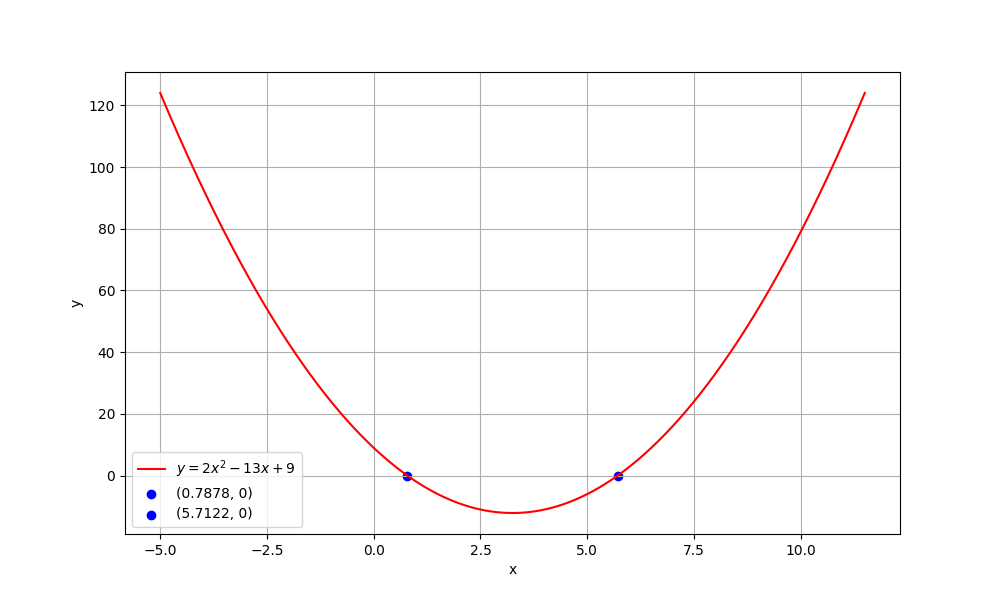
\includegraphics[width=0.8\columnwidth]{figs/fig.png}
   \caption{Graph of $y = 2x^2-13x+2$}
   \label{stemplot}
\end{figure}
\end{frame}
\end{document}

